

\chapter{Joint Executions}

\label{ch:jointexec}

TODO: ref branching in "semantics of deliberation in IndiGolog", and CATs in [find this ref]

Third, planning in the situation calculus involves building situation
terms representing the sequence of actions to be performed. Situations
inherently impose a total ordering on actions, and cannot represent
the independent execution of actions by different agents. Executing
a plan built using situation terms therefore requires constant synchronisation
among the agents. Even if such synchronicity is achievable, it is
usually not desirable.

However, some representational limits of the situation calculus make
it unsatisfactory, by itself, for rich multi-agent domains. The fundamental
unit of reasoning, and the output of the ConGolog execution planning
process, is the \emph{situation}: a complete, ordered history of all
actions that have occurred in the world. Working with a total ordering
over actions is far from ideal in a multi-agent setting as it requires
constant synchronization between the agents. This severely limits
the potential for concurrency in the system. Moreover, such synchronization
may not even be possible if agents are unaware of the actions performed
by others. Multi-agent applications of the situation calculus thus
invariably assume that all actions performed are public, available
to all agents for the purposes of reasoning and synchronization. This
is clearly unrealistic in many domains.

This chapter shows how these apparent limitations of the situation
calculus can in fact be overcome, by developing a formalism for explicitly
working with only a partial ordering on actions. We take inspiration
from a model of concurrent computation known as \emph{prime event}
\emph{structures} \citep{npw79event_structures}, which are partially-ordered
branching sequences of events.

We define a \emph{joint execution} as a particular kind of prime event
structure that is rich enough to capture the concurrent execution
of independent actions, including actions with sensing results, but
restricted enough that it can be unambiguously reduced back to situation
terms for the purposes of reasoning. To demonstrate the utility of
the approach, we show how a team of agents can cooperate to plan and
perform an execution of a shared ConGolog program in an asynchronous,
partially observable domain.

Rather than assuming that all actions are public, we leverage recent
work by \citep{kelly07sc_know_obs} to axiomatize the conditions under
which an agent will be aware of the occurrence of an action. Joint
executions are restricted such that whenever action $a_{1}$ must
be performed before action $a_{2}$, the agent performing $a_{2}$
is able to observe the occurrence of $a_{1}$. Synchronization thus
occurs by observing the actions of other agents. If this is not possible,
yet synchronization is needed to ensure correctness, then construction
of the joint execution will fail. In general, whether an action is
enabled at any stage of execution can be determined using only the
information available to the agent who is to perform it.

Joint executions thus allow us to capture the actions that a team
of agents are to perform in service of some shared task, without requiring
constant synchronization between the agents, and without assuming
that agents know all the actions that have been performed, while utilizing
existing reasoning methods based on full situation terms. This is
a significant increase in expressiveness over existing approaches
to modeling multi-agent teams in the situation calculus.


\section{Background}


\subsection{Event Structures}

To tackle cooperative execution in a multi-agent setting, we have
adopted a model of concurrent computation known as \emph{event structures,}
introduced in \citep{npw79event_structures}. The particular variant
we are interested in are \emph{prime event structures}, canonically
defined as a four-tuple:\[
(\mathcal{V},\prec,\#,\gamma)\]
 where: $\mathcal{V}$ is a set of events; $\gamma$ is a function
assigning a label to each event; $\prec$ is the \emph{enabling} relation,
a strict partial order on events; and $\#$ is the \emph{conflict}
relation, a binary symmetric relation that is inherited through enablers:\[
\forall i,j,k\in V:i\#j\wedge i\prec k\rightarrow k\#j\]


A \emph{configuration} is a sequence of events consistent with $\prec$
in which no pair of events conflict. Each configuration thus represents
a potential partial run of execution of the system.

For convenience, we will define our prime event structures using a
slightly different form:\[
(\mathcal{V},ens,alts,\gamma)\]


Here $ens(i)$ assigns to each event $i\in\mathcal{V}$ a finite set
of other events that are its direct \emph{enablers}, meaning that
event $i$ can only occur after all the events in $ens(i)$ have occurred.
Similarly $alts(i)$ assigns to each event a set of direct \emph{alternatives},
meaning that only one of the events in $\{i\}\cup alts(i)$ can occur
during execution of the system. The enabling relation $i\prec j$
is then the transitive closure of $i\in ens(j)$, and $\#$ is the
smallest relation satisfying:\[
\forall i,j\in V:[\exists i',j'\in V:i'\preceq i\wedge j'\preceq j\wedge i\in alts(j)]\rightarrow i\#j\]
 Considered in this way, event structures form a directed acyclic
graph of the events that could occur during execution of the system.
As shown in \citep{pratt91modeling_conc_with_geom}, it is straightforward
to convert these structures into a kind of finite automaton for efficient
execution.


\section{Joint Executions}

\label{sec:Joint-Execs}


\subsection{Independent Actions}

As discussed in Section \ref{sec:Background}, posing queries in the
situation calculus requires a full situation term, which means a total
order on all actions that have occurred. The first step towards providing
only a \emph{partial} order on the actions to be performed is, therefore,
to capture the conditions under which actions can be performed out
of order without invalidating the results of the reasoning process.

Define \emph{independent} actions, identified by $indep(a_{1},a_{2})$,
as those that can be performed in either order without affecting what
holds in the resulting situation. Formally, they must satisfy the
following restrictions (where $\mathcal{P}$ and $\mathcal{F}$ are
meta-variables ranging over predicate and functional fluents respectively):

\begin{itemize}
\item $Poss(a_{1},s)\equiv Poss(a_{1},do(a_{2},s))$ 
\item $Poss(a_{2},s)\equiv Poss(a_{2},do(a_{1}s))$ 
\item $\mathcal{P}(do(a_{1},do(a_{2},s)))\equiv\mathcal{P}(do(a_{2},do(a_{1},s)))$\\
 for all predicate fluents $\mathcal{P}(s)$ 
\item $\mathcal{F}(do(a_{1},do(a_{2},s)))=r\equiv\mathcal{F}(do(a_{2},do(a_{1},s)))=r$\\
 for all functional fluents $\mathcal{F}(s)$ 
\end{itemize}
Whether actions are independent can be deduced from the description
of the action theory, or (as currently in our implementation) indicated
explicitly by the programmer.

We will say that two situations are \emph{equivalent} if they are
identical up to transposition of pairs of adjacent independent actions.
A straightforward case analysis on the definition of the regression
operator shows that for equivalent situations $s_{1}$ and $s_{2}$,
$\mathcal{D}\models\phi(s_{1})$ iff $\mathcal{D}\models\phi(s_{2})$.

This notion of equivalence can be extended by macro expansion to histories
in the obvious manner, with the analogous result that $\mathcal{D}\cup\mathbf{sensed}[\sigma_{1}]\models\phi(\mathbf{end}[\sigma_{1}])$
iff $\mathcal{D}\cup\mathbf{sensed}[\sigma_{2}]\models\phi(\mathbf{end}[\sigma_{2}])$.


\subsection{Joint Executions}

We define a \emph{joint execution} as a special kind of prime event
structure with the following components:\[
(\mathcal{A},\mathcal{O},ens,alts,\gamma,<)\]
 It contains two disjoint sets of events: \emph{action} events $\mathcal{A}$
representing the actions to be performed, and \emph{outcome} events
$\mathcal{O}$ representing the possible outcomes of each action.
For each action event $a\in\mathcal{A}$, its enablers $ens(a)$ is
a set of outcome events, its alternatives $alts(a)$ is empty, and
its label $\gamma(a)$ is the action to be performed. For each outcome
event $o\in\mathcal{O}$, $ens(o)$ is a single action event for which
it is a possible outcome, $alts(o)$ is the set of all other outcome
events $o'$ such that $ens(o')=ens(o)$, and $\gamma(o)$ is an outcome
as produced by the $Out(a,s)$ function for the action $\gamma(ens(o))$.

A simple example of a joint execution is shown in Figure \ref{fig:example-je}.
Here action $act1$ has two possible outcomes, which enable different
actions $act2$ and $act3$.

%
\begin{figure}
\framebox{%
\begin{minipage}[t][1\totalheight]{1\columnwidth}%
\textsf{\textbf{\tiny 
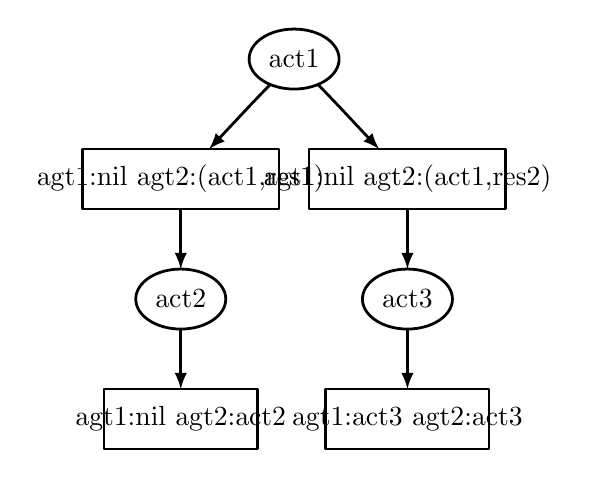
\begin{tikzpicture}[>=latex,join=bevel,scale=0.60]
  \pgfsetlinewidth{1bp}
%
\pgfsetcolor{black}
  % Edge: n1 -> n2
  \draw [->] (113bp,219bp) .. controls (104bp,210bp) and (93bp,198bp)  .. (76bp,180bp);
  % Edge: n1 -> n3
  \draw [->] (141bp,219bp) .. controls (150bp,210bp) and (161bp,198bp)  .. (178bp,180bp);
  % Edge: n4 -> n5
  \draw [->] (59bp,72bp) .. controls (59bp,64bp) and (59bp,55bp)  .. (59bp,36bp);
  % Edge: n6 -> n7
  \draw [->] (195bp,72bp) .. controls (195bp,64bp) and (195bp,55bp)  .. (195bp,36bp);
  % Edge: n2 -> n4
  \draw [->] (59bp,144bp) .. controls (59bp,136bp) and (59bp,127bp)  .. (59bp,108bp);
  % Edge: n3 -> n6
  \draw [->] (195bp,144bp) .. controls (195bp,136bp) and (195bp,127bp)  .. (195bp,108bp);
  % Node: n1
\begin{scope}
  \pgfsetstrokecolor{black}
  \draw (127bp,234bp) ellipse (27bp and 18bp);
  \draw (127bp,234bp) node {act1};
\end{scope}
  % Node: n2
\begin{scope}
  \pgfsetstrokecolor{black}
  \draw (118bp,180bp) -- (0bp,180bp) -- (0bp,144bp) -- (118bp,144bp) -- cycle;
  \draw (59bp,162bp) node {agt1:nil agt2:(act1,res1)};
\end{scope}
  % Node: n3
\begin{scope}
  \pgfsetstrokecolor{black}
  \draw (254bp,180bp) -- (136bp,180bp) -- (136bp,144bp) -- (254bp,144bp) -- cycle;
  \draw (195bp,162bp) node {agt1:nil agt2:(act1,res2)};
\end{scope}
  % Node: n4
\begin{scope}
  \pgfsetstrokecolor{black}
  \draw (59bp,90bp) ellipse (27bp and 18bp);
  \draw (59bp,90bp) node {act2};
\end{scope}
  % Node: n5
\begin{scope}
  \pgfsetstrokecolor{black}
  \draw (105bp,36bp) -- (13bp,36bp) -- (13bp,0bp) -- (105bp,0bp) -- cycle;
  \draw (59bp,18bp) node {agt1:nil agt2:act2};
\end{scope}
  % Node: n6
\begin{scope}
  \pgfsetstrokecolor{black}
  \draw (195bp,90bp) ellipse (27bp and 18bp);
  \draw (195bp,90bp) node {act3};
\end{scope}
  % Node: n7
\begin{scope}
  \pgfsetstrokecolor{black}
  \draw (244bp,36bp) -- (146bp,36bp) -- (146bp,0bp) -- (244bp,0bp) -- cycle;
  \draw (195bp,18bp) node {agt1:act3 agt2:act3};
\end{scope}
%
\end{tikzpicture}

}}{\tiny {} }%
\end{minipage}}

\caption{ A simple joint execution. Elliptical nodes are action events, box
nodes are outcome events. }


\label{fig:example-je} 
\end{figure}


A joint execution has one additional component over a standard prime
event structure: a \emph{total} order on events $<$ that is consistent
with the partial order $\prec$ induced by the enabling relation.
We will use this to perform reasoning by assuming that events occur
in the fixed order given by $<$, and placing restrictions on the
joint execution to ensure this assumption is acceptable. In practice,
$<$ will be determined by the order of insertion of events.

An \emph{outcome set} is a minimal set of non-conflicting outcome
events; that is, a set of events $e\subset\mathcal{O}$ satisfying:\begin{gather*}
\forall o_{1},o_{2}\in e\,:\,\neg(o_{1}\#o_{2})\\
\forall o_{1},o_{2}\in e\,:\, o_{1}\not\prec o_{2}\,\wedge o_{2}\not\prec o_{1}\end{gather*}


Recall that a \emph{configuration} is a partial run of execution of
the prime event structure. Clearly any configuration ending in an
outcome event corresponds to a unique history, as it is a set of alternating
actions and their outcomes. We call the \emph{histories} of an outcome
set, denoted $hists(e)$, the set of all configurations that contain
all elements of $e$, and end in an event from $e$. The unique history
of an outcome set that is consistent with $<$ will be denoted $hist(e)$.

We say that an outcome set $e_{1}$ \emph{covers} a set \emph{$e_{2}$,}
denoted by $e_{1}\sqsubseteq e_{2}$, if every event in $e_{1}$ is
either also in $e_{2}$, or precedes something in $e_{2}$. Every
history in $hists(e_{2})$ will have a prefix in $hists(e_{1})$.
This defines a partial ordering on outcome sets:\[
e_{1}\sqsubseteq e_{2}\,\equiv\,\forall o_{1}\in e_{1}:\,\,\exists o_{2}\in e_{2}:\,\, o_{1}\preceq o_{2}\]


Let $max(e)$ denote the maximal element of an outcome set with respect
to the total order $<$. A \emph{branch}, denoted $b$, is a special
case of an outcome set that meets the following additional requirement:\[
\forall i<max(b):\,\, i\in b\,\oplus\,(\exists i'\in b:\,\, i\#i'\,\vee\, i\prec i')\]


That is, every event less than the maximal element of $b$ is either
in the branch, conflicts with something in the branch, or precedes
something in the branch. A branch thus identifies a unique outcome
for each action event that is ordered below $max(b)$.


\subsection{Restrictions on Joint Executions}

\label{sub:Restrictions}

We now impose several restrictions on the structure of a joint execution,
to ensure they are suitable for representing the actions to be performed
by a team of agents.\\


\textbf{(R1) Independent events have independent actions:}\\
 Joint executions are restricted such that the following holds for
all action events $a_{1},a_{2}\in\mathcal{A}$:\[
a_{1}<a_{2}\,\rightarrow\, a_{1}\prec a_{2}\,\vee\, a_{1}\#a_{2}\,\vee\, indep(\gamma(a_{1}),\gamma(a_{2}))\]


In words: if event $a_{2}$ is after $a_{1}$ in the total order,
but the execution allows them to be performed in either order, then
the corresponding actions must be independent.

With this restriction, the histories given by $hists(b)$ will differ
from each other only by transposition of independent actions, making
them equivalent to the unique history $hist(b)$. It is thus possible
to determine whether a formula holds after the execution of a given
branch, using the query:\[
\mathcal{D}\cup\mathbf{sensed}[hist(b)]\models\phi(\mathbf{end}[hist(b)])\]


This is a key point and is worth re-iterating: regardless of the precise
order in which events are executed, any history that contains all
events on a branch $b$, and that ends in an event from $b$, is equivalent
to the unique history of $b$ generated by the total order. This allows
us to plan using execution branches rather than histories or situation
terms.\\


\textbf{(R2) Actions are enabled by a unique branch:}\\
 We restrict the enabling set for each action event to be a branch,
rather than an arbitrary set of outcome events. In practice this means
that when inserting a new action into the joint execution, one must
specify the branch to which it belongs. This restriction allows us
to determine what holds immediately before an event $a\in\mathcal{A}$
becomes enabled, using $hist(ens(a))$. Given that the action $\gamma(a)$
is possible after $ens(a)$, then when $a$ becomes enabled it will
remain possible until it is performed. Moreover, any events that occur
after it is enabled but before it is performed will not interfere
with its effects, as these actions must be independent of $\gamma(a)$.
\\


\textbf{(R3) All possible outcomes are considered:}\\
 Clearly planning requires that all possible outcomes of an action
be considered. For each action event $a\in\mathcal{A}$, and each
possible outcome $r$ of that action, if:\begin{multline*}
D\cup\mathbf{sensed}[hist(ens(a))]\not\,\models\,\\
Out(\gamma(a),\mathbf{end}[hist(ens(a))])\neq r\end{multline*}


then there must be a corresponding outcome event:\[
\exists o\in E:\,\, ens(o)=\{a\}\,\wedge\,\gamma(o)=r\]


\textbf{(R4) Actions are enabled by observable events:}\\
 If an action is to be enabled by an outcome event $o$ produced by
another agent, it is clearly necessary that the agent performing the
action be able to observe the occurrence of $o$. Otherwise, it has
no way of synchronizing its actions with those of its teammate. Let
$actor(a)$ be the agent responsible for performing an action event
$a$, then we require that:\[
\forall o\in ens(a):\,\,\gamma(o)[actor(a)]\neq nil\]


\textbf{(R5) Overlapping views enable identical actions:}\\
 To ensure that the joint execution can actually be carried out by
the agents, there must be no confusion about whether a particular
action is enabled. Lifting the function $view$ to operate on sets
of histories in the obvious way, then:\[
view(actor(a),\, hists(ens(a)))\]
 gives the set of all local histories after which $actor(a)$ is required
to perform the action $\gamma(a)$. However, since the agent has only
a local viewpoint, it may be the case that some other outcome set
can produce an identical local history.

Say that two branches overlap, denoted $overlaps(b,b')$, if they
could produce an identical local history from the perspective of a
given agent:\[
view(agt,hists(b))\,\cap\, view(agt,hists(b'))\,\neq\varnothing\]


Then the \emph{minimal overlapping set} for $b$, from the perspective
of $agt$, is the set of all $b'$ satisfying:\[
overlaps(agt,b,b')\wedge\neg\exists b''\left[overlaps(agt,b,b'')\wedge b''\sqsubset b'\right]\]


This set captures all branches that the agent could potentially confuse
for $b$. To ensure there is no confusion about whether an action
is enabled, for each $a\in\mathcal{A}$, every $b$ in the minimal
overlapping set of $ens(a)$ for $actor(a)$ must enable an event
$a'$ with identical action $\gamma(a')=\gamma(a)$. This ensures
that the agent's local information is always enough to know when it
should perform an action. While it may not know precisely which \emph{event}
is enabled, it will know enough to determine the specific \emph{action}
that it must perform.


\subsection{Planning with Joint Executions}

Our implementation of an execution planning system uses joint executions
as an abstract data type that can be built up one event at a time,
one branch at a time. For a particular branch $b$, the state of the
world is reasoned about using standard regression techniques over
$hist(b)$, to determine the next action to perform. This action is
then be inserted into the joint execution to extend the branch.

Inserting a new action event requires specifying the action to be
performed, the branch on which to insert it, and a set of existing
events on that branch that must precede it. The code managing the
joint execution determines all possible outcomes of the action and
adds them as outcome events, returning a new branch for each outcome.
It also ensures that the restrictions in Section \ref{sub:Restrictions}
are satisfied, which can involve forcing an ordering between potentially
concurrent events to ensure independence (R1) or synchronization (R4),
or adding actions to other branches that the acting agent cannot distinguish
from the current one (R5). If the restrictions cannot be met, insertion
fails and the planner must backtrack to find a different action.

The intricacies of synchronization between agents in the face of partial
observability are thus hidden from the planning algorithm itself,
automatically managed by the construction of a joint execution.


\subsection{Summary}

In this section we have defined a \emph{joint execution} as a prime
event structure with some additional restrictions. We contend that
such structures are highly suitable for planning the actions to be
performed by a team in service of some shared task, such as executing
a shared ConGolog program.

On one hand, joint executions are restricted enough to be practical
for such use. Like the situation terms or conditional action trees
used in previous approaches, prime event structures are purely reactive
(equivalent to a kind of finite automaton) and can be executed without
further deliberation. They are restricted to ensure that whenever
an agent is required to perform an action, it is able to determine
this using only its local information. Each branch of execution can
be easily converted into a situation term for the purposes of reasoning,
and can be extended one action at a time.

Joint executions are also significantly more flexible than previous
approaches. They allow independent actions to be performed without
synchronization, in any order. The agents need never know precisely
what actions have been executed, only those that enable them to perform
their next action. Synchronization is automatically achieved when
required by explicitly reasoning about what actions each agent can
observe, rather than requiring that all actions be public.

To demonstrate the utility of these structures, we have implemented
an interpreter for multi-agent ConGolog programs that produces joint
executions as its output. In the next section, we highlight the key
aspects of our implementation and give an example of the output it
produces.


\section{Implementation}

\label{sec:Implementation}

Our implementation%
\footnote{available at {[}identifying information omitted]%
} of a ConGolog execution planner utilizes the Mozart programming system,
which implements the Oz language \citep{vanroy99mozart} rather than
the traditional use of Prolog. As we shall see, Mozart's strong support
for distributed logic programming allows the team of agents to share
the planning workload with almost no additional code.

To make things more concrete, Figure \ref{fig:plan-output} shows
the output of our system when run on the $MakeSalad$ example of Figure
\ref{fig:makesalad-program}. Since all actions in this program have
a single outcome, the outcome events have been suppressed for brevity.

In this domain there are three agents, but only two knives are available.
The agents must therefore synchronize their use of these resources.
Actions are taken to be independent if they deal with different objects.
As seen in Figure \ref{fig:plan-output}, the use of a partial order
structure facilitates parallelism between the agents, with each processing
a different ingredient and only synchronizing on the availability
of the required resources. There is no need for processing actions,
such as $mix$ and $chop$, to be publicly observable. This execution
is maximally concurrent given the constraints of the domain, and is
clearly a significant improvement over totally ordered sequences of
actions as produced by existing systems.

In the following subsections, we briefly highlight some key aspects
of our implementation.


\subsection{Program Steps}

While the ability to determine whether actions are independent is
necessary in constructing partially-ordered executions of a ConGolog
program, it is not sufficient. Actions might have an order imposed
on them directly by the program (for example by the sequence construct
$a_{1};a_{2}$). The program may require that some additional conditions
are true immediately prior to executing an action (for example to
satisfy a test construct $\phi?$), which could be falsified by an
otherwise independent action.

To ensure that the dependencies between actions reflect the needs
of the program being executed, we augment our implementation of the
$Trans$ predicate to keep additional information about what transitions
were made. A \emph{step} object has the following attributes:

\begin{itemize}
\item action: the action performed in that step, or $nil$ if it is an internal
program transition 
\item test: an additional fluent formula that must hold immediately before
performing the step 
\item thread: a sequence of 'l' and 'r' characters indicating the concurrent
thread in which the step is performed 
\item outcome: the outcome of performing the action. 
\end{itemize}
%
\begin{figure}
\framebox{%
\begin{minipage}[t][1\totalheight]{1\columnwidth}%
\textsf{\textbf{\tiny 
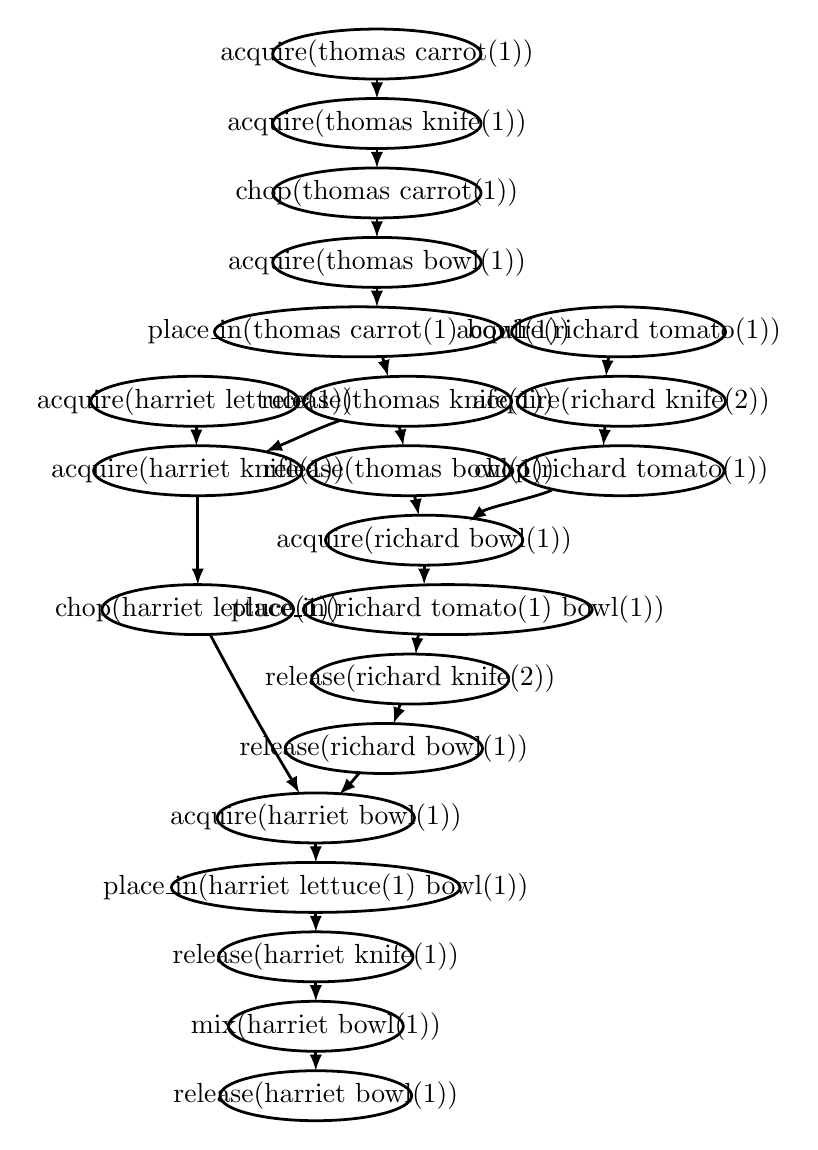
\begin{tikzpicture}[>=latex,join=bevel,scale=0.50]
  \pgfsetlinewidth{1bp}
%
\pgfsetcolor{black}
  % Edge: n0 -> n6
  \draw [->] (196bp,750bp) .. controls (196bp,749bp) and (196bp,748bp)  .. (196bp,736bp);
  % Edge: n2 -> n8
  \draw [->] (363bp,550bp) .. controls (363bp,549bp) and (362bp,547bp)  .. (361bp,536bp);
  % Edge: n6 -> n10
  \draw [->] (196bp,700bp) .. controls (196bp,699bp) and (196bp,698bp)  .. (196bp,686bp);
  % Edge: n8 -> n12
  \draw [->] (360bp,500bp) .. controls (360bp,499bp) and (360bp,497bp)  .. (359bp,486bp);
  % Edge: n10 -> n14
  \draw [->] (196bp,650bp) .. controls (196bp,649bp) and (196bp,648bp)  .. (196bp,636bp);
  % Edge: n14 -> n16
  \draw [->] (196bp,600bp) .. controls (196bp,599bp) and (196bp,598bp)  .. (196bp,586bp);
  % Edge: n16 -> n18
  \draw [->] (200bp,550bp) .. controls (200bp,549bp) and (201bp,547bp)  .. (204bp,536bp);
  % Edge: n18 -> n20
  \draw [->] (212bp,500bp) .. controls (212bp,499bp) and (213bp,497bp)  .. (215bp,486bp);
  % Edge: n18 -> n22
  \draw [->] (169bp,504bp) .. controls (152bp,498bp) and (138bp,491bp)  .. (116bp,482bp);
  % Edge: n4 -> n22
  \draw [->] (66bp,500bp) .. controls (66bp,499bp) and (66bp,498bp)  .. (66bp,486bp);
  % Edge: n20 -> n24
  \draw [->] (223bp,450bp) .. controls (223bp,449bp) and (224bp,447bp)  .. (226bp,436bp);
  % Edge: n12 -> n24
  \draw [->] (322bp,454bp) .. controls (308bp,448bp) and (276bp,442bp)  .. (263bp,432bp);
  % Edge: n22 -> n26
  \draw [->] (67bp,450bp) .. controls (67bp,435bp) and (67bp,413bp)  .. (67bp,386bp);
  % Edge: n24 -> n28
  \draw [->] (230bp,400bp) .. controls (230bp,399bp) and (230bp,398bp)  .. (230bp,386bp);
  % Edge: n28 -> n30
  \draw [->] (226bp,350bp) .. controls (226bp,349bp) and (225bp,347bp)  .. (224bp,336bp);
  % Edge: n30 -> n32
  \draw [->] (213bp,300bp) .. controls (212bp,299bp) and (212bp,297bp)  .. (208bp,286bp);
  % Edge: n32 -> n34
  \draw [->] (184bp,251bp) .. controls (181bp,248bp) and (179bp,245bp)  .. (169bp,235bp);
  % Edge: n26 -> n34
  \draw [->] (76bp,350bp) .. controls (88bp,327bp) and (111bp,285bp)  .. (132bp,250bp) .. controls (133bp,248bp) and (134bp,247bp)  .. (140bp,236bp);
  % Edge: n34 -> n36
  \draw [->] (152bp,200bp) .. controls (152bp,199bp) and (152bp,198bp)  .. (152bp,186bp);
  % Edge: n36 -> n38
  \draw [->] (152bp,150bp) .. controls (152bp,149bp) and (152bp,148bp)  .. (152bp,136bp);
  % Edge: n38 -> n40
  \draw [->] (152bp,100bp) .. controls (152bp,99bp) and (152bp,98bp)  .. (152bp,86bp);
  % Edge: n40 -> n42
  \draw [->] (152bp,50bp) .. controls (152bp,49bp) and (152bp,48bp)  .. (152bp,36bp);
  % Node: n0
\begin{scope}
  \pgfsetstrokecolor{black}
  \draw (196bp,768bp) ellipse (75bp and 18bp);
  \draw (196bp,768bp) node {acquire(thomas carrot(1))};
\end{scope}
  % Node: n2
\begin{scope}
  \pgfsetstrokecolor{black}
  \draw (370bp,568bp) ellipse (77bp and 18bp);
  \draw (370bp,568bp) node {acquire(richard tomato(1))};
\end{scope}
  % Node: n4
\begin{scope}
  \pgfsetstrokecolor{black}
  \draw (65bp,518bp) ellipse (75bp and 18bp);
  \draw (65bp,518bp) node {acquire(harriet lettuce(1))};
\end{scope}
  % Node: n6
\begin{scope}
  \pgfsetstrokecolor{black}
  \draw (196bp,718bp) ellipse (75bp and 18bp);
  \draw (196bp,718bp) node {acquire(thomas knife(1))};
\end{scope}
  % Node: n8
\begin{scope}
  \pgfsetstrokecolor{black}
  \draw (372bp,518bp) ellipse (75bp and 18bp);
  \draw (372bp,518bp) node {acquire(richard knife(2))};
\end{scope}
  % Node: n10
\begin{scope}
  \pgfsetstrokecolor{black}
  \draw (196bp,668bp) ellipse (75bp and 18bp);
  \draw (196bp,668bp) node {chop(thomas carrot(1))};
\end{scope}
  % Node: n12
\begin{scope}
  \pgfsetstrokecolor{black}
  \draw (372bp,468bp) ellipse (74bp and 18bp);
  \draw (372bp,468bp) node {chop(richard tomato(1))};
\end{scope}
  % Node: n14
\begin{scope}
  \pgfsetstrokecolor{black}
  \draw (196bp,618bp) ellipse (75bp and 18bp);
  \draw (196bp,618bp) node {acquire(thomas bowl(1))};
\end{scope}
  % Node: n16
\begin{scope}
  \pgfsetstrokecolor{black}
  \draw (183bp,568bp) ellipse (104bp and 18bp);
  \draw (183bp,568bp) node {place\_in(thomas carrot(1) bowl(1))};
\end{scope}
  % Node: n18
\begin{scope}
  \pgfsetstrokecolor{black}
  \draw (218bp,518bp) ellipse (75bp and 18bp);
  \draw (218bp,518bp) node {release(thomas knife(1))};
\end{scope}
  % Node: n20
\begin{scope}
  \pgfsetstrokecolor{black}
  \draw (219bp,468bp) ellipse (73bp and 18bp);
  \draw (219bp,468bp) node {release(thomas bowl(1))};
\end{scope}
  % Node: n22
\begin{scope}
  \pgfsetstrokecolor{black}
  \draw (67bp,468bp) ellipse (75bp and 18bp);
  \draw (67bp,468bp) node {acquire(harriet knife(1))};
\end{scope}
  % Node: n24
\begin{scope}
  \pgfsetstrokecolor{black}
  \draw (230bp,418bp) ellipse (71bp and 18bp);
  \draw (230bp,418bp) node {acquire(richard bowl(1))};
\end{scope}
  % Node: n26
\begin{scope}
  \pgfsetstrokecolor{black}
  \draw (67bp,368bp) ellipse (69bp and 18bp);
  \draw (67bp,368bp) node {chop(harriet lettuce(1))};
\end{scope}
  % Node: n28
\begin{scope}
  \pgfsetstrokecolor{black}
  \draw (247bp,368bp) ellipse (104bp and 18bp);
  \draw (247bp,368bp) node {place\_in(richard tomato(1) bowl(1))};
\end{scope}
  % Node: n30
\begin{scope}
  \pgfsetstrokecolor{black}
  \draw (220bp,318bp) ellipse (71bp and 18bp);
  \draw (220bp,318bp) node {release(richard knife(2))};
\end{scope}
  % Node: n32
\begin{scope}
  \pgfsetstrokecolor{black}
  \draw (201bp,268bp) ellipse (71bp and 18bp);
  \draw (201bp,268bp) node {release(richard bowl(1))};
\end{scope}
  % Node: n34
\begin{scope}
  \pgfsetstrokecolor{black}
  \draw (152bp,218bp) ellipse (71bp and 18bp);
  \draw (152bp,218bp) node {acquire(harriet bowl(1))};
\end{scope}
  % Node: n36
\begin{scope}
  \pgfsetstrokecolor{black}
  \draw (152bp,168bp) ellipse (104bp and 18bp);
  \draw (152bp,168bp) node {place\_in(harriet lettuce(1) bowl(1))};
\end{scope}
  % Node: n38
\begin{scope}
  \pgfsetstrokecolor{black}
  \draw (152bp,118bp) ellipse (70bp and 18bp);
  \draw (152bp,118bp) node {release(harriet knife(1))};
\end{scope}
  % Node: n40
\begin{scope}
  \pgfsetstrokecolor{black}
  \draw (152bp,68bp) ellipse (63bp and 18bp);
  \draw (152bp,68bp) node {mix(harriet bowl(1))};
\end{scope}
  % Node: n42
\begin{scope}
  \pgfsetstrokecolor{black}
  \draw (152bp,18bp) ellipse (69bp and 18bp);
  \draw (152bp,18bp) node {release(harriet bowl(1))};
\end{scope}
%
\end{tikzpicture}

}}%
\end{minipage}}

\caption{ Joint execution for $MakeSalad(bowl(1))$, showing significant concurrency
between agents }


\label{fig:plan-output} 
\end{figure}


We call a sequence of such steps a \emph{run}, which can be converted
to a history by taking just the action and outcome attributes. The
procedure implementing $Trans$ takes a program and a run as input,
returning a new program and new step of execution. As an example consider
the code in Figure \ref{fig:trans-code}, implementing the test operator
and the concurrency operator from equation \ref{eqn:trans_conc_orig}.

%
\begin{figure}
\framebox{%
\begin{minipage}[t][1\totalheight]{1\columnwidth}%
{\scriptsize \verbatiminput{listings/jointexec/ConGolog.oz}}%
\end{minipage}}

\caption{ Partial code for $Trans$ predicate }


\label{fig:trans-code} 
\end{figure}


Note that whenever the procedure descends through the left side of
a concurrency operator it pushes an 'l' onto the step's {}``thread''
attribute, and each descent through the right side pushes an 'r'.
Two steps can be said to come from different threads as long as neither
{}``thread'' attribute is a prefix of the other.

We say that two steps are \emph{ordered} if any of the following holds:
their action terms are not independent; ones thread is a prefix of
the other; ones action falsifies the test condition associated with
the other. When building a joint execution, ordered steps are forced
to be executed in the order they were generated by the planner, while
unordered steps may be performed independently.


\subsection{Planning Procedure}

The code for planning a joint execution from a given ConGolog program
is shown in Figure \ref{fig:planning-code}. The main procedure is
$MakePlan$, a recursive procedure that operates on a list of branches-in-progress
of the form $(D,R,B)$. Here $B$ is a branch in the joint execution
under construction, $D$ is the program remaining to be executed on
that branch, and $R$ is the run of program steps performed on that
branch so far.

%
\begin{figure}
\framebox{%
\begin{minipage}[t][1\totalheight]{1\columnwidth}%
{\scriptsize \verbatiminput{listings/jointexec/Planner.oz}}%
\end{minipage}}

\caption{ Code for main planning loop }


\label{fig:planning-code} 
\end{figure}


%
\begin{figure}
\framebox{%
\begin{minipage}[t][1\totalheight]{1\columnwidth}%
{\scriptsize \verbatiminput{listings/jointexec/psearch.oz}}%
\end{minipage}}

\caption{ Code to run planning procedure in parallel }


\label{fig:parallel-search} 
\end{figure}


Each iteration of the planning loop proceeds as follows. The procedure
$FindOpenBranch$ updates each branch to account for events that were
added since it was last processed (some may have been added automatically
to satisfy restriction (R5)), then searches the list to find a branch
for which $Final(D,R)$ does not hold. If all branches are final,
planning can terminate. Otherwise, the procedure $FindTrans1$ is
called to find a new step of execution for that branch. The action
is inserted into the joint execution, which returns a list of new
branches, one for each possible outcome of the action. Each of these
outcomes is added to the list of branches, and the loop is started
again.

Of particular interest is the procedure $FindTrans1$, which uses
the encapsulated search functionality of Mozart to yield possible
next steps according to an estimate of their potential for concurrency.
The procedure $LP.yieldOrdered$ yields the solutions of the given
search context, sorted using the procedure $CompareSteps$. This procedure
(not shown) gives preference to steps that can be performed concurrently
with as many existing actions as possible.


\subsection{Distributing the Planning Workload}

A primary motivation in using Mozart/Oz for our implementation is
its strong support for distributed logic programming. Utilizing Mozart's
parallel search functionality \citep{Schulte00constraint_services},
the planning workload can be transparently distributed between the
agents in the team.

Figure \ref{fig:parallel-search} shows the necessary code, which
should be executed by one of the agents. The planning procedure is
encapsulated in a \emph{functor}, a portable code object. A parallel
search object is then created, which uses an ssh connection to spawn
remote computations on each of the three agents (identified by their
DNS names). The object is asked to provide a single solution, which
is then written to a file in the graphviz 'dot' format for display
(resulting in Figure \ref{fig:plan-output}).

For the simple example shown in this chapter, parallel plan search
does not demonstrate a significant time saving since almost no backtracking
is required to reach a solution. For more difficult problems, significant
gains can be expected.


\section{Related and Future Work}

\label{sec:Related-Work}

The idea of having a shared ConGolog program that is executed by a
team of agents is used with considerable success in \citep{Ferrein2005readylog},
where the variant Readylog is used to coordinate and control a RoboCup
soccer team. Their domain satisfies the assumption that all actions
are public, so they can afford to produce totally ordered plans. The
techniques developed in this chapter would generalize such an approach
to a wider variety of domains (although \citep{Ferrein2005readylog}
includes some decision theoretic aspects that are not present in our
work).

There has also been significant work using the situation calculus
in settings where each agent has its own control program \citep{shapiro02casl}.
The behavior of the overall system is specified as the concurrent
combination of each agent's program, $\delta_{1}||\delta_{2}||\dots$,
and ConGolog is used to verify that the system satisfies certain constraints
(e.g. safety or liveness properties). Again, this cannot handle partial
observability of actions since all reasoning is based on a full situation
term. We believe the joint execution formalism could be helpful in
such settings, by permitting synchronization only when actions are
observable by the agents.

An alternate approach to the problem of partial observability is the
language TeamGolog developed in \citep{farinelli07team_golog}, where
agents explicitly synchronize through communication and a shared state.
By contrast, our approach constructs synchronization implicitly by
reasoning about the actions that can be observed by each agent. This
has the advantage of requiring no changes to the form or semantics
of the agents' control program, but the disadvantage that joint execution
construction may fail if too many actions are unobservable. It would
be interesting to combine these approaches by automatically incorporating
explicit communication when implicit synchronization is not possible.

Several authors have introduced operators for expressing partial orderings
between actions into the ConGolog language itself, for example \citep{son00htn_golog}.
While this is unquestionably useful for specifying behavior, the \emph{output}
from such systems is still a totally ordered sequence of actions and
thus maintains the limitations of existing systems when actually performing
the execution in a multi-agent setting.

There is, of course, an extensive body of work on partial-order planning
in the context of goal-based planning. Unsurprisingly, the joint execution
structure we develop here has deep similarities to the structures
used in conditional partial-order planners such as \citep{peot92conditional_nonlinear}.
It is, however, intentionally specific to the situation calculus.
We make no use of many concepts common in partial-order goal-based
planning (causal links, threats, conflicts, etc) because we do not
deal explicitly with goals, but with steps generated by an underlying
transition semantics. Our approach can be considered roughly equivalent
to \emph{deordering} of a totally-ordered plan as described in \citep{backstrom99reordering},
except performed during plan construction rather than as a post-processing
step. \bibliographystyle{plainnat} \bibliographystyle{plainnat}

